\chapter{FET projects and social media}
This chapter presents an overview of the presence of FET projects on social media. Ut enim ad minim veniam, quis nostrum exercitationem ullam corporis suscipit laboriosam, nisi ut aliquid ex ea commodi consequatur. Quis aute iure reprehenderit in voluptate velit esse cillum dolore eu fugiat nulla pariatur. Excepteur sint obcaecat cupiditat non proident, sunt in culpa qui officia deserunt mollit anim id est laborum.

\section{Considered channels} 
There exist disparate channels suitable for communication purposes. Those offering the widest audience are provided by the web. Examples are websites and social media. For this reason, FET projects consider the internet as one of the main pillars of their communication strategy.

Different approaches can be considered to assess the use of online communication channels made by FET projects. One quantitative estimate is provided by the fraction of projects active on specific platforms. For this thesis, the following communication channels were considered:   

\begin{description}
 \item [Website] The website is the online channel offering the highest degree of freedom to the owner. It allows the owner to personalise the content, the overall structure and the graphic impact.
 \item [Facebook] Facebook is the most used social media. It offers direct interaction among users and activities are recorded. Nevertheless, it is mainly designed for free time.  
 \item [Twitter] Twitter is very effective for short science-related communication. However, it requires high posting rates and offers less personal interaction compared to Facebook.
 \item [Linkedin] LinkedIn is ideal for professional content and enables the creation of closed groups. Two drawbacks are the limited interaction among users and the outreach within the groups.
 \item [YouTube] 
\end{description}

\begin{itemize}
 \item YouTube
 \item ResearchGate
\end{itemize}

Lorem ipsum dolor sit amet, consectetur adipisci elit, sed eiusmod tempor incidunt ut labore et dolore magna aliqua. Ut enim ad minim veniam, quis nostrum exercitationem ullam corporis suscipit laboriosam, nisi ut aliquid ex ea commodi consequatur. Quis aute iure reprehenderit in voluptate velit esse cillum dolore eu fugiat nulla pariatur. Excepteur sint obcaecat cupiditat non proident, sunt in culpa qui officia deserunt mollit anim id est laborum.

\begin{figure}[!t] 
 \begin{center}
 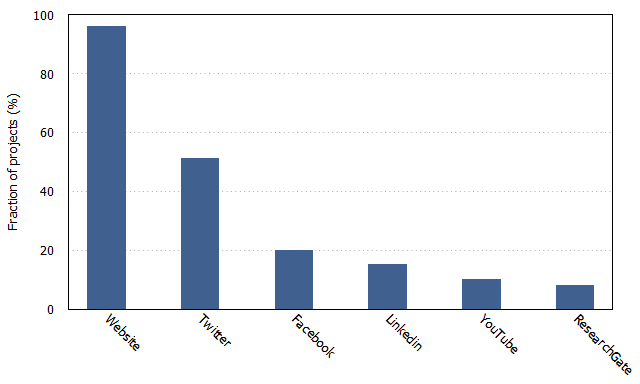
\includegraphics[scale=0.4]{Images/Social_media.png}
 \caption{Duration and allocated budget of Europe's Research and Innovation programmes (also known as Framework Programmes, FP). Budgets are expressed in billion Euros.}
 \label{FP_funds}
 \end{center}
\end{figure}